\scanpage{29}
local structure of $X_j$ along an $X_i$
(with the induced stratification of type $I_{ij}$)
is ``cubical''
(corner of a cube of
dimension $n=\operatorname{card}S$)

\figure{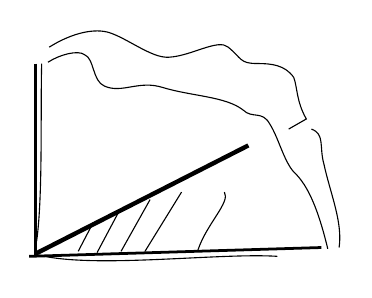
\begin{tikzpicture}[x=0.016cm,y=-0.016cm]
\draw[line width=1pt] (21,35)--(21,187);
\draw (26,35) .. controls (25,75) and (27,140) .. (22,176);
\draw[line width=1pt] (16,188)--(248,181);
\draw (24,187) .. controls (68,198) and (167,185) .. (213,188);
\draw (31,34) .. controls (40,28) and (55,24) .. (60,28)
.. controls (68,31) and (66,49) .. (76,53)
.. controls (90,59) and (103,48) .. (122,54)
.. controls (145,61) and (172,61) .. (186,72)
.. controls (193,79) and (201,72) .. (207,83)
.. controls (214,94) and (218,112) .. (226,121)
.. controls (238,132) and (246,153) .. (253,182);
\draw (32,22) .. controls (48,12) and (65,7) .. (78,10)
.. controls (93,14) and (113,31) .. (127,30)
.. controls (145,29) and (166,15) .. (174,22)
.. controls (185,31) and (183,35) .. (197,35)
.. controls (208,35) and (219,36) .. (226,46)
.. controls (229,54) and (228,65) .. (236,79)
--(222,87);
\draw (240,87) .. controls (251,91) and (246,101) .. (250,115)
.. controls (255,138) and (265,161) .. (262,181);
\draw[line width=1.6pt] (21,186)--(190,100);
\draw (55,184)--(67,161);
\draw (70,185)--(87,153);
\draw (89,184)--(112,143);
\draw (108,184)--(137,137);
\draw (150,183) .. controls (157,162) and (176,145) .. (171,137);
\end{tikzpicture}}

The \deleted{condition} \inserted{c)} \unsure{imply|implies} that if $j'$ is
a predecessor of $j$, and if $k\in I$ is $\le j$
but not $\le j'$, and if there exists
an $i$ bounded above by $k$ and $j'$, \uline{then}
$k'=\operatorname{Inf}(k,j')$ exists, and $k'$ is
a predecessor of $k$.

\diagram{\begin{tikzcd}[column sep=small,row sep=small]
& j' \arrow[r,leftrightarrow,"\mathrm{predecessor}"'] \arrow[d,phantom,"{\rotatebox{90}{$\leq$}}" description] & j \arrow[d,phantom,"{\rotatebox{90}{$\leq$}}" description] \\
& k' \arrow[r,leftrightarrow] & k \\
i \arrow[uur,hook] \arrow[urr,hook] & &
\end{tikzcd}}

(It suffices to see that in
an ordered set of the form $\mathcal P(\unsure{\sigma|F})$,
the infima exist (it is the intersection) and if
$j'\subset j=j'\amalg\{\alpha\}$, and $k\in j$ but not $k\subset j'$,
then \deleted{$\unsure{k\ne k'}$} $k=k'\amalg\{\alpha\}$ with $k'=k\cap j'$, ..)
\margin{$\sigma$ finite set}

This being so, let us consider the diagram
\diagram{\begin{tikzcd}
X_{j'} \arrow[r,hook] & X_j \\
X_{k'} \arrow[u] \arrow[r,hook] & X_k \arrow[u]
\end{tikzcd}}
where the vertical arrows, by hypothesis $\unsure{1^\circ)|16)}$,
are boundary embeddings. This being so, one
sees \inserted{(by b,c)} that \deleted{$(X_k\longrightarrow X_{\unsure{j}}$.}
$(X_k,X_{k'})\mathbin{-}(X_j,X_{j'})$
\margin{28}
